\chapter[Les mèmes Internet, objets numériques culturels]{Les mèmes Internet, objets numériques culturels}

Afin de mener à bien cette étude, nous avons choisi de nous intéresser à un objet numérique particulier : les \textit{mèmes Internet}. Courts messages se propageant rapidement sur la Toile, les mèmes proposent une illustration pertinente des discursivités multiples qui prennent place dans les échanges en ligne. Plus que de simples blagues de potache, nous verrons ici comment ces constructions collectives éphémères laissent parfois des traces symboliques qui structurent le milieu numérique qui les produit. Nous présenterons tout d{\textquoteright}abord la notion controversée de \textit{mème}, définie d{\textquoteright}abord comme une unité minimale de diffusion des cultures. Nous verrons ensuite comment ce concept teinté d{\textquoteright}un évolutionnisme peu convaincant flotte depuis sa création en marge de la littérature scientifique. En introduisant ensuite les \textit{mèmes Internet}, nous observerons le fort regain de popularité dont a bénéficié ce mot ces dix dernières années\textit{. }Nous envisagerons ensuite le rôle des mèmes Internet - et à plus forte raison des technologies numériques - en resituant leur étude dans la perspective historique plus large des questionnements sur la formation de mémoires collectives. En interrogeant notamment la notion de {\textquotedblleft}performativité{\textquotedblright}, nous verrons comment les pratiques \textit{d{\textquoteright}énonciation }qui entourent les mèmes Internet forment une pratique rhétorique et une activité symbolique importante dans l{\textquoteright}actualisation et l{\textquoteright}échange de signes. Enfin, nous détaillerons les processus discursifs entourant les mèmes en proposant une catégorisation selon l{\textquoteright}intention des énoncés, comme prélude méthodologique à notre démonstration.

\section[Les mèmes : définitions et histoire ]{Les mèmes : définitions et histoire } 

Le dictionnaire d{\textquoteright}Oxford\footnote{ D{\textquoteright}après \textit{British \& Words English} publié par Oxford University Press en 2014, \ \url{http://www.oxforddictionaries.com/definition/english/meme}, consulté le 24 Février 2014 à 21:50} donne deux définitions du mot \textit{mème }: 

\begin{quote}
    \textit{Meme} (n.)

    \begin{enumerate}
        \item Un élément d{\textquoteright}une culture ou système de comportement passé d{\textquoteright}un individu à un autre par imitation ou par d{\textquoteright}autres moyens non-génétiques.
        \item Une image, vidéo, morceau de texte, etc., la plupart du temps de nature \ \ humoristique, qui est copié(e) et propagé(e) rapidement par les utilisateurs \ \ d{\textquoteright}Internet, souvent après avoir été modifié(e).
    \end{enumerate}

\end{quote}

 Cette définition nous renseigne sur l{\textquoteright}usage de ce terme, en le définissant à la fois comme un élément culturel transmissible et comme une forme particulière de contenus diffusé sur Internet. En nous appuyant sur son évolution dans la littérature, nous allons tout d{\textquoteright}abord essayer de voir comment les deux versants de ce concept se sont historiquement articulés et à plus forte raison comment cette articulation peut nous servir pour comprendre les phénomènes à l{\textquoteright}{\oe}uvre dans les réseaux sociaux en Chine. 

\subsection[La mémétique : une éthologie culturelle teinté d{\textquoteright}évolutionnisme]{La mémétique : une éthologie culturelle teinté d{\textquoteright}évolutionnisme}

Le premier usage du concept de \textit{mème} est souvent attribué au biologiste Richard Dawkins dans son livre \textit{Le Gène égo\"iste }(1976). Dawkins s{\textquoteright}inspire des théories évolutionnistes de l{\textquoteright}éthologie moderne pour proposer le \textit{mème} comme un élément moléculaire de la culture qui permettrait sa transmission, semblable au gène des individus biologiques. Considéré comme une \textit{{\guillemotleft}~unité d{\textquoteright}information culturelle qui peut être copiée, située dans le cerveau~{\guillemotright}} \citep{Blackmore2001}, le mème serait la fondation de pratiques culturelles qui évolueraient selon des variations de la sélection naturelle. Représenté comme une {\guillemotleft}~\textit{unité distincte de la pensée {\guillemotright}} \citep{Dawkins1989}, le concept se fonde sur l{\textquoteright}analogie entre les processus de transmission culturelle et génétique: \textit{{\textquotedblleft}Cultural transmission is analogous to genetic transmission in that, although basically conservative, it can give rise to a form of evolution{\textquotedblright} }(p.72)\textit{.} Cette approche éthologique de la culture considère donc le \textit{mème} à la fois comme un élément transmissible et un facteur de transmission doté de la capacité de se reproduire lui-même. élément actif, le mème serait donc un \textit{{\guillemotleft}~gène égo\"iste {\guillemotright} }agissant de manière isolée et distincte, spécificité d{\textquoteright}une {\textquotedblleft}culture{\textquotedblright}. Plus encore, son but unique serait sa propre pérennisation par sa propagation de cerveau en cerveau \citep{Blackmore1997}. Il agit donc comme un agent culturel possédant une forme de volonté propre pour se propager. Souvent représenté gr\^ace à l{\textquoteright}image du virus, il donne l{\textquoteright}idée d{\textquoteright}une propagation de la culture sous forme de contamination avec en arrière-plan une lutte pour la survie et la fécondité des idées. Le mème est un {\textquotedblleft}réplicateur culturel{\textquotedblright}, une extension à part entière du vivant au-delà du biologique (Bloom, 2002). 

 Le québécois Fernand Dumont définit la culture comme cette \textit{{\guillemotleft}~maison o\`u l{\textquoteright}on habite ensemble~{\guillemotright} }\citep{Dumont1993}. N{\oe}ud dans une topologie sociale, le mème pourrait donc également se présenter comme un point d{\textquoteright}entrée, une porte entrouverte vers ce lieu o\`u d{\textquoteright}autres sont déjà passés et se trouvent encore. Le mème devenu particule culturelle définit un seuil, ce lieu de passage si particulier qui \textit{{\guillemotleft}~fonde les espaces~{\guillemotright}} \citep{Bonnin2000} et invite ou interdit d{\textquoteright}entrer. Comme on enlève ces chaussures au dojo et qu{\textquoteright}on sonne à la porte, les mèmes sont peut-être à envisager comme des rites de franchissement de seuils culturels, pratiques de liaison du vivre-ensemble politique d{\textquoteright}Arendt \citep{Arendt2001} . Pour le gène comme pour le mème, il ne s{\textquoteright}agit pas de considérer la fonction mécanique d{\textquoteright}un {\textquotedblleft}réplicateur{\textquotedblright} mais d{\textquoteright}observer l{\textquoteright}altération qui se déroule lors de son actualisation pour en comprendre les limites et le rôle. La présence \textit{in potentia }d{\textquoteright}une unité culturelle identique ne constitue pas nécessairement une réalité in-formante pour des groupes sociaux ou des individus \citep{Lissack2004}. Les sciences de la communication ont largement étudié depuis 50 ans les modalités de transmission des informations. Les études sur la réception notamment ont bien montré qu{\textquoteright}il ne suffisait pas qu{\textquoteright}un message soit émis pour être décodé et compris \citep{Liebes1990}. Déjà avec Shannon et Weaver \citep{Jakobson1960}, l{\textquoteright}environnement exprimé par le concept de\textit{ bruit }vient altérer largement les phénomènes de transmission tout au long de leurs diffusions \citep{Attali1978}. La mémétique, faute d{\textquoteright}étude de cas conséquentes et d{\textquoteright}applications théoriques réelles \citep{Jouxtel2014} a subi de nombreux revers conceptuels en s{\textquoteright}appuyant notamment sur l{\textquoteright}image peu crédible d{\textquoteright}une transmission par réplication quasi-mécanique. Ignorant la dimension poétique des actes de transmission, cette vision mécaniste issue d{\textquoteright}une rationalisation excessive reflète pourtant les écueils non-dits des approches scientifiques modernes. Thierry Bardini dans son livre \textit{Junkware }(2011) effectue une recherche extensive sur les discussions et considérations qui entourent la partie non-codante de l{\textquoteright}ADN appelée \textit{{\textquotedblleft}junk ADN{\textquotedblright}}. Analysant les discussions dans les publications scientifiques, il montre comment plus de 80\% des éléments structurant l{\textquoteright}ADN ont été très tôt étiquetés comme {\textquotedblleft}bruit{\textquotedblright} puis {\textquotedblleft}junk{\textquotedblright}, car il était impossible d{\textquoteright}identifier leur participation active au codage de protéines. La métaphore de ce \textit{{\textquotedblleft}junk non-codant{\textquotedblright} }si envahissant et la relative facilité avec laquelle nous nous permettons de l{\textquoteright}ignorer démontre la nécessité d{\textquoteright}une approche renouvelée des phénomènes complexes du vivant, et notamment de ceux de la transmission culturelle. Déjà clairement identifiées dans les études en communication, les fonctions non-langagières notamment sont indispensables au bon déroulement d{\textquoteright}un acte de langage. Ainsi si la suppression du bruit est souvent un préalable méthodologique pour l{\textquoteright}étude scientifique, elle peut souvent fausser l{\textquoteright}approche expérimentale et les conclusions théoriques en refusant d{\textquoteright}admettre sa partialité. L{\textquoteright}étude des mèmes est encore largement en quête de reconnaissance scientifique et si la construction théorique permettant d{\textquoteright}isoler des éléments culturels pour l{\textquoteright}étude parait intéressante, elle manque d{\textquoteright}une réelle prise sur l{\textquoteright}observation et l{\textquoteright}analyse par l{\textquoteright}étude de cas notamment. La fermeture dès 2005 du \textit{Journal of Memetics}, parution de référence de la discipline naissante est annoncé dès 2002 par un article de B. Edmonds \citep{Jouxtel2014}. Intitulé \textit{Three Challenges for the Survival of Memetics}, l{\textquoteright}article\textit{ }exhorte les chercheurs intéressés à produire ce que Edmonds juge comme le minimum indispensable pour gagner la reconnaissance des milieux scientifiques : \textit{{\textquotedblleft}a conclusive case-study; a theory for when memetic models are appropriate; and a simulation of the emergence of a memetic process.{\textquotedblright}} \citep{Edmonds2002}.  
En effet, il parait impossible d{\textquoteright}assoir scientifiquement la légitimé du concept en se fondant uniquement sur une analogie de phénomènes. Si le mème a donc raté sa cible dans le domaine scientifique, son acception plus récente sous la forme de contenus Internet a néanmoins redonné au concept une nouvelle vie dans la culture populaire. Dans le même temps, ce sens renouvelé a permis de définir précisément un domaine d{\textquoteright}application idéal et a permis l{\textquoteright}émergence de nouvelles études dont nous allons maintenant discuter. 

\subsection[ Mèmes Internet : définition, littérature et exemples]{Mèmes Internet : définition, littérature et exemples}

Contrairement au concept éthérique de mème présenté dans la partie précédente, la définition des \textit{mèmes Internet }est de prime abord plus pragmatique. Il s{\textquoteright}agit de courts messages faits de texte, image, vidéo ou de son gagnant rapidement une forte popularité sur Internet en étant partagés, commentés, réappropriés puis transformés lors de leur diffusion. L{\textquoteright}utilisation du terme \textit{mème Internet }pour décrire la diffusion de messages ne recouvre pas nécessairement la dimension évolutive et culturelle du concept initial de Dawkins, mais garde l{\textquoteright}idée générale d{\textquoteright}une circulation {\guillemotleft}~virale~{\guillemotright} d{\textquoteright}idées parmi des groupes d{\textquoteright}individus\footnote{ \textit{"The meaning is not that far away from the original. It's anything that goes viral."}, Dawkins interviewé par le magazine \textit{Wired} \url{http://www.wired.co.uk/news/archive/2013-06/20/richard-dawkins-memes}, consulté le 12/08/2013 à 7h53 GMT+8}. Le concept de mème a très fortement gagné en popularité avec cette nouvelle acception. En 2012, il a notamment été sélectionné parmi les 10 mots les plus marquants de l{\textquoteright}année par le prestigieux dictionnaire américain Merriam-Webster. Ce choix a été motivé par la très forte popularité sur Internet des images parodiques du politicien Mitt Romney après une bourde lors d{\textquoteright}une intervention télévisée aux Etats-Unis\footnote{ \textit{{\textquotedblleft}Words of the year 2012{\textquotedblright}}, Merriam-Webster \url{http://www.merriam-webster.com/info/2012words.htm} consulté le 25 Février 2014 à 19:01 GMT+1}. Ainsi, le mot \textit{mème }dans une acception que nous prendrons ici soin de nommer \textit{mème} \textit{Internet} est aujourd{\textquoteright}hui entré dans le vocabulaire commun du Web. De nombreux sites spécialisés~(knowyourmeme.org, quickmeme.org, memefest.org, etc) ont vu le jour avec comme mission d{\textquoteright}archiver et de collecter ces pièces de la culture web. Un des plus anciens mèmes Internet est certainement l{\textquoteright}usage des émoticônes ou smileys, ces petites figures qui servent à exprimer des émotions dans le contexte d{\textquoteright}oralité écrite d{\textquoteright}Internet. Apparu dans les premiers jours du réseau Internet, les émoticônes répondent à un besoin d{\textquoteright}expression non-verbale dans la communication en ligne. Très simples à utiliser ou à modifier, les \textit{smileys }connaissent une popularité rapide et se diversifient partout autour de la toile.  

\begin{figure}[ht]
    \centering
    

    \begin{quote}
    19-Sep-82 11:44~~~ Scott E~ Fahlman~~~~~~~~~~~~ :-)

    From: Scott E~ Fahlman {\textless}Fahlman at Cmu-20c{\textgreater}

    ~
    
    I propose that the following character sequence for joke markers:

    ~~~~~~~ 

    :-)

    ~~~~~~~ 
    
    Read it sideways.~ Actually, it is probably more economical to mark things that are NOT jokes, given current trends.~ For this, use

    ~~~~~~~ 

    :-(

    \end{quote}
    \caption[la première mention du smiley par Scott Fahlman]{19 Septembre 1982 : la première mention du smiley par Scott Fahlman\protect\footnotemark, que l’on retrouve quelques jours plus tard sur les mailing lists les plus utilisées de l’époque : Arpanet\protect\footnotemark  et Usenet \protect\footnotemark}
    \label{fig:smiley-story}
\end{figure}

\footnotetext{D’après \url{http://www.cs.cmu.edu/~sef/Orig-Smiley.htm} archive consultée le 10 Août 2013 à 09 :15 GMT+8}
\footnotetext{Usenet mailing list \url{https://groups.google.com/forum/\#!msg/net.works/dzzAYYz9fYM/m6DZBY5ZpzUJ} sarchive consultée le 10 Août 2013 à 09 :25 GMT+8}
\footnotetext{Usenet mailing list \url{https://groups.google.com/forum/?hl=en\#!topic/net.news/tywzPO0NOtw} archive consultée le 10 Août 2013 à 09 :20 GMT+8}

L{\textquoteright}usage des émoticones s{\textquoteright}est aujourd{\textquoteright}hui largement répandu, notamment chez les adolescents et jeunes adultes (D Derks, Bos, \& Von Grumbkow, 2007). Une récente étude a même montré que les zones du cerveau stimulées par la vue d{\textquoteright}émoticones étaient similaires à celles stimulées lors de la vue d{\textquoteright}un visage, indiquant un ancrage symbolique profond de l{\textquoteright}usage de ces signes \citep{Churches2014}. Des émoticônes singuliers se sont également développés dans différentes langues pour exprimer des sentiments particuliers, propres au langage et à ses modes d{\textquoteright}expression. Le caractère idéographique des langues chinoise et japonaise se prête particulièrement à ces jeux de dessin langagier. En chinois, le plus célèbre exemple est sans doute le caractère [56E7?] (jiong4) qui représente en langue ancienne une fenêtre d{\textquoteright}o\`u provient la lumière et signifie {\guillemotleft}~lumineux~{\guillemotright}. Sa ressemblance avec une figure humaine (un émoticône) a fait renaitre ce caractère désuet qui signifie désormais qu{\textquoteright}un utilisateur est agacé, embarrassé ou même choqué. La conjonction {\textquotedbl}[56E7?]rz{\textquotedbl} a même été inventé : [56E7?]représentant la tête et \textit{rz} le corps agenouillé d{\textquoteright}une personne ; elle signifie l{\textquoteright}échec et le désespoir. Cette particularité des langues asiatiques donnent à l{\textquoteright}émoticône un rôle central dans la communication en ligne qui se traduit dans le design des interfaces. Les réseaux sociaux chinois proposent tous par défaut de multiples jeux d{\textquoteright}émoticônes disponibles pour l{\textquoteright}utilisateur qui communiquent ainsi très rapidement en images.  

\begin{figure}[h]
    \centering
    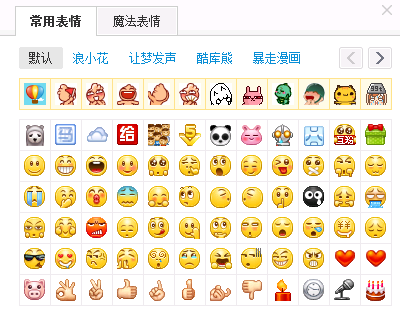
\includegraphics[width=4.1669in,height=3.278in]{figures/chap2/chapitre2-img1.png}
    \caption[Un jeu d{\textquoteright}émoticônes de Weibo]{Un jeu d{\textquoteright}émoticônes sur \url{weibo.com} -- Consulté le 10 Aout 2013 à 10:00 GMT+8}
    \label{fig:emoticons-weibo}
\end{figure}


L{\textquoteright}exemple de l{\textquoteright}émoticone illustre donc la manière dont un élément visuel et langagier vient constituer les pratiques en ligne, en relation proche avec la culture et le lieu qui l{\textquoteright}a fait na\^itre. 

Il est difficile de définir un mème a priori par la nature de son contenu. Néanmoins, la structure de la diffusion d{\textquoteright}un message peut nous permettre de le décrire comme un mème. Reproduisant en grande partie le cycle de vie classique d{\textquoteright}une information comme une rumeur ou une \textit{news, }les mèmes possèdent des modes de diffusion en ligne assez déterminés et prévisibles. La plupart du temps, ils sont mis en circulation sur un petit nombre de sites spécialisés, avant d{\textquoteright}être repris dans une première phase par un assez petit nombre d{\textquoteright}utilisateurs qui se charge de les publier sur les réseaux sociaux \citep{Bauckhage2011}. Les réseaux sociaux agissent alors comme une chambre d{\textquoteright}écho, qui détermine si le {\textquotedblleft}proto-mème{\textquotedblright} encore en devenir deviendra mème ou restera simple message isolé. Durant cette phase souvent nommée \textit{adoption,} le mème entre en concurrence avec d{\textquoteright}autres informations sur les réseaux sociaux o\`u les utilisateurs sont sans cesse \ sollicités par d{\textquoteright}autres informations (Davenport \& Beck, 2001). Si l{\textquoteright}attention générée par le mème auprès des utilisateurs atteint un pic suffisamment important, il faut environ 2h30 pour que les mèmes rejoignent les pages des médias plus traditionnels en commen\c{c}ant par les blogs, puis les sites d{\textquoteright}information (Leskovec, Backstrom, \& Kleinberg, 2009) . Ensuite, l{\textquoteright}attention envers le mème décroit fortement et rapidement. La présence épisodique de citations maintient l{\textquoteright}existence du mème apparente dans des groupes définis \citep{Buchel2012}.

\begin{figure}[h]
    \centering
    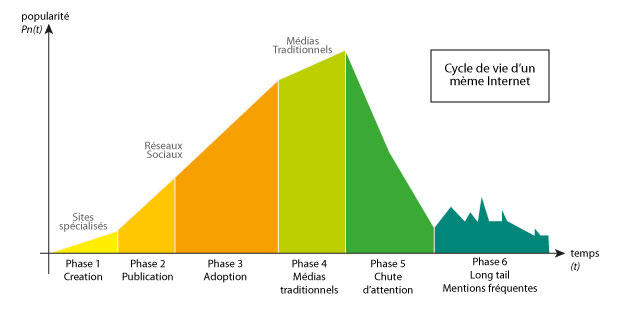
\includegraphics[width=6.2559in,height=3.1559in]{figures/chap2/chapitre2-img2.jpg}
    \caption[Cycle de vie d{\textquoteright}un mème Internet]{Cycle de vie d{\textquoteright}un mème Internet -Clément Renaud - 2013}
    \label{fig:meme-lifecycle}
\end{figure}

L{\textquoteright}évolution du volume de la diffusion permet donc de définir un mème Internet. Néanmoins, il est impossible de donner une estimation du volume minimum pour devenir {\textquotedblleft}mème{\textquotedblright} tant ce chiffre dépend de la population étudiée : il existe des mèmes à très forte diffusion comme le smiley ; d{\textquoteright}autres mèmes se diffusent seulement au sein de groupes d{\textquoteright}individus restreints sans s{\textquoteright}étendre en-dehors. Ainsi, certains mèmes peuvent avoir connu une diffusion très importante dans un groupe, mais rester absolument inconnu du reste de l{\textquoteright}Internet. Une étude de 2012 comparant la diffusion de nombreux mèmes sur Twitter montre que les utilisateurs tendent à choisir les mèmes selon la structure de leur réseau social et le moment d{\textquoteright}exposition, produisant ainsi une grande hétérogénéité des mèmes dans le réseau (Weng, Flammini, Vespignani, \& Menczer, 2012). Ainsi, il est hasardeux d{\textquoteright}essayer de décrire le concept de mème par son contenu tant les sujets et les discussions varient. 

Quelques éléments d{\textquoteright}ordre grammaticaux peuvent néanmoins être observés dans la forme que prennent les contenus, appelé parfois {\textquotedblleft}véhicule{\textquotedblright} du mème. Les mèmes qui sont diffusés les plus largement sont composés d{\textquoteright}images et de vidéo. L{\textquoteright}économie d{\textquoteright}attention très limitée de l{\textquoteright}Internet et les modes de lecture sur écran dans un contexte d{\textquoteright}abondance d{\textquoteright}informations font que l{\textquoteright}on privilégie souvent les médias visuels sur le texte \citep{Goldhaber2006}. Un autre élément important est la facilité avec laquelle un message peut être approprié par un utilisateur qui veut le modifier ou tout simplement le diffuser dans le réseau. L{\textquoteright}existence des mèmes est en effet largement conditionnée par la possibilité d{\textquoteright}une diffusion à moindre co\^ut et effort pour l{\textquoteright}utilisateur final, la plupart du temps non-rémunéré. Ici on voit émerger une structure visuelle caractéristique du mème : une image accompagnée d{\textquoteright}une légende écrite en caractères blancs détourés de noir, ou de caractères blancs sur fond noir. L{\textquoteright}utilisation de haut contraste de couleur dans les typographies permet de faire apparaitre très efficacement des légendes juxtaposées à l{\textquoteright}image.


\begin{figure}[h]
    \centering
    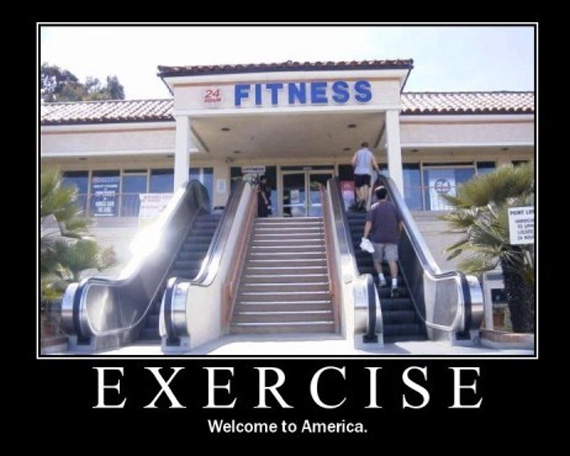
\includegraphics[width=3.6335in,height=2.9114in]{figures/chap2/chapitre2-img3.jpg}
    
\includegraphics[width=2.2559in,height=2.9449in]{figures/chap2/chapitre2-img4.jpg}
    \caption[Exemples de mèmes internet]{Exemples de mèmes Internet, d{\textquoteright}après \url{http://knowyourmeme.org}, consulté le 12/08/2013 à 10 :01 GMT+8}
    \label{fig:memes-examples}
\end{figure}


L{\textquoteright}usage d{\textquoteright}images légendées est une des formes les plus communes pour les mèmes Internet, en particulier ceux de nature comique ou absurde. La mise en place de sites permettant de générer rapidement ce type d{\textquoteright}images légendées (memegenerator.com, mememachine.com, etc.) renforcent l{\textquoteright}unité formelle des mèmes sur l{\textquoteright}Internet, ou plutôt sur l{\textquoteright}Internet anglophone et francophone notamment. En effet, on constate que cette forme typique du mème ne se retrouve pas sur l{\textquoteright}Internet chinois qui utilise plus volontiers des montages d{\textquoteright}images ou des jeux de mots, avec davantage de diversité dans les formes que peuvent prendre les différents mèmes.

\section[Mème, mémoire collective et culture]{Mème, mémoire collective et culture}
\subsection[La mémoire comme trace]{La mémoire comme trace}

Si le concept de mème est souvent considéré comme très récent, on peut néanmoins le resituer facilement dans le vaste paysage des travaux sur la mémoire collective qui ont existé depuis le XIXème siècle \citep{Laurent1999}. Max Stirner dans son livre \textit{The Ego and Its Own }\citeyear{Stirner1995} énonce déjà l{\textquoteright}idée que les individus sont sujets à la circulation de concepts issus de souvenirs communs ou illusoires, comme notamment le nationalisme et la religion. Le logicien Bertrand Russell reprend par la suite dans son livre \textit{The Analysis of Mind } \citeyear{Russell1921} les travaux sur la mémoire et l{\textquoteright}évolution sociale du physiologiste allemand Richard Semon \citeyear{Semon1923}. Utilisant le concept central de \textit{mneme} (du grec 
%\textit{$\mu \nu \text{\textgreek{'h}}\mu \eta $ }  
mneme, mémoire), Semon travaille sur l{\textquoteright}idée de \textit{{\textquotedblleft}traces mnésiques{\textquotedblright} }laissées par les diverses expériences au niveau cellulaire comme au niveau de l{\textquoteright}organisme tout entier. La psychanalyse a également cherché à saisir cette distance impalpable entre expérience et organisme en interrogeant les marques laissées par les souvenirs. Pour Freud comme pour Semon, {\textquotedblleft}l{\textquoteright}appareil psychique{\textquotedblright} de la mémoire se constitue sous la forme de {\textquotedblleft}traces{\textquotedblright}, qu{\textquoteright}il se refuse néanmoins à localiser dans des zones spécifiques du cerveau. Lacan après lui suggèrera que la perception et la mémoire des expériences se structurent dans le langage lui-même, seul outil de connaissance du monde. Depuis les dix dernières années, plusieurs découvertes dans le domaine de la neurologie viennent corroborer cette idée que la mémoire existe sous forme de traces. Les travaux autour de la \textit{plasticité neuronale }montrent notamment l{\textquoteright}existence de la mémoire sous la forme de connections, relations ténues ancrées dans notre réseau neuronal global \citep{Magistretti2008}.  

\begin{table}[ht]
    \centering
    \begin{tabulary}{\textwidth}{L|C C C}
        
        ~ & t=1  & t=2  & t=3 \\[2ex]
        
        \hline \\ [-1.5ex]
    
        Freud  & expérience  & perception  & Traces mnémiques et psychiques \\[3ex]

        Lacan & expérience (signifié)  &   perception (signifié)  &   Signifiant (traces structurées dans le langage) \\[3ex]

        Neurosciences &  expérience & Perception & Traces synaptiquesassemblages de neurones \\[3ex]

    \end{tabulary}

    \caption{ Etapes constituantes de la mémoire - Convergence entre la trace psychique et synaptique \citep{Ansermet2004} }
\end{table}

Ces disciplines s{\textquoteright}intéressent majoritairement à l{\textquoteright}étude de la constitution d{\textquoteright}une mémoire individuelle, ne nous livrant que peu de clés pour comprendre les éléments qui font qu{\textquoteright}une mémoire devient commune. Le paléontologiste Leroi Gourhan propose dans son livre \textit{L{\textquoteright}homme et la Matière} \citeyear{Leroi-Gourhan1971} de considérer que les humains possèdent trois formes de mémoire : une mémoire individuelle sensible, stockée dans les organes du corps ; une mémoire héritée génétiquement, stockée dans l{\textquoteright}ADN ; et une troisième forme de mémoire, transmise de générations en générations : la \textit{technologie}. Dans sa lecture de Leroi-Gourhan, Stiegler (1998b) explique comment \textit{l{\textquoteright}objet technologique} porte en lui les traces des expérimentations, réussites et échecs passés, mémoire cumulative de temps et de sociétés passées, à la fois héritée et commune, transmissible par son usage.

\begin{table}[ht]
    \begin{tabulary}{\textwidth}{L|C C}
        \centering
        \textbf{Forme de mémoire} &  \textbf{Contenu}  & \textbf{Stockage} \\[3ex]
        \hline \\ [-1.5ex]
        génétique  &  Particularités héritées des ancêtres   &  DNA \\[3ex]
        
        épigénétique   &  Mémoire sensible de l’expérience personnelle   &  Organes, nerfs, cerveau \\[3ex]
        
        technologique  &  Pratiques de la vie quotidienne en société (usages) & Objets technologiques \\[3ex]
    \end{tabulary}
    \caption{Les trois formes de mémoire d{\textquoteright}après Leroi-Gourhan et Stiegler}
\end{table}


\subsection[Diffusion de mèmes et structuration d{\textquoteright}une mémoire collective]{Diffusion de mèmes et structuration d{\textquoteright}une mémoire collective}
La relation entre mémoire humaine et mémoire technologique est au centre de notre étude. La technologie a depuis toujours été considérée comme une mémoire extérieure. Dans \textit{Phèdre, }Platon raconte l{\textquoteright}histoire du roi égyptien Thamous recevant en cadeau du dieu Thot l{\textquoteright}écriture, le remède (\textit{pharmakon) }qui devait \textit{{\textquotedblleft}soulager la science et la mémoire{\textquotedblright} }(Platon, 274e). Le roi Thamous, effrayé par cette nouvelle technologie de la mémoire qu{\textquoteright}est l{\textquoteright}écriture se voit saisi de l{\textquoteright}angoisse d{\textquoteright}une perte de cette mémoire. Avec la fin de cette oralité, la disparition de la méthode active des antiques thé\^atres de la mémoire au profit d{\textquoteright}une mémoire technologique inerte et extérieure à soi pourrait-t-elle sceller l{\textquoteright}avènement d{\textquoteright}une nouvelle bêtise? Aujourd{\textquoteright}hui, l{\textquoteright}importance grandissante des bases de données et de connaissances soulèvent encore une fois les mêmes questions, toujours irrésolues. Nicolas Carr constate notamment que \textit{{\textquotedblleft}l{\textquoteright}Internet nous rend stupide{\textquotedblright}} et que son usage répété entraine une baisse drastique de nos facultés de concentration \citep{Carr2010}. A l{\textquoteright}ère du Big Data et de l{\textquoteright}expansion sans fin de notre mémoire numérique, la constitution de nos bases de données interroge notre construction d{\textquoteright}une mémoire collective. Les mèmes Internet, d{\textquoteright}abord gravés dans les disques durs des serveurs, viennent être actualisés par ceux qui les partagent, les commentent, jouent avec et se les approprient. L{\textquoteright}exemple de l{\textquoteright}Internet chinois nous montre la volatilité de cette mémoire numérique, artefact historiographique d{\textquoteright}une culture soumise au bon-vouloir des administrateurs du réseau. Le \textit{Manifeste de l{\textquoteright}Archiviste} publié par Yuk Hui \citeyear{Hui2014} s{\textquoteright}ouvre sur l{\textquoteright}angoissante interrogation deleuzienne :  

\begin{quote}
Un nouvel archiviste est nommé dans la ville. Mais est-il à proprement parler nommé ?
N'est-ce pas sur ses propres instructions qu'il agit ? 
\citep{Deleuze1972a}.
\end{quote}

L{\textquoteright}existence et l{\textquoteright}usage quotidien des bases de données questionnent chaque jour l{\textquoteright}assujettissement des symboles de notre mémoire à l{\textquoteright}objet technologique, à la fois béquille, prothèse et maquillage postiche de notre détestable devenir bête. L{\textquoteright}étude des mèmes Internet nous offre ici une fenêtre pour porter notre regard sur ces objets dont le corps scellée dans les profondeurs glacées des \textit{data centers }nous parvient en dansant, d{\textquoteright}abord sur nos écrans puis dans un coin de notre tête. Avec l{\textquoteright}usage répété des technologies et de l{\textquoteright}écriture numérique, les frontières entre milieu numérique et mémoire collective s{\textquoteright}estompent pour laisser entrevoir un enchevêtrement de silicium, d{\textquoteright}idées et de chair, constitutifs de notre savoir moderne. 

Poursuivant l{\textquoteright}idée d{\textquoteright}une archéologie du présent introduite par Foucault, il s{\textquoteright}agit donc de documenter les processus par lesquels ces obscurs habitants des bases de données viennent laisser leurs traces pour constituer des bribes de nos mémoires collectives. Maurice Halbwachs dans son vaste travail aborde les fa\c{c}ons dont l{\textquoteright}histoire structure l{\textquoteright}être-ensemble des groupes humains. En disant que \textit{"l'histoire de notre vie fait partie de l'histoire en général"}\citep{Halbwachs1947}, il identifie une mémoire autobiographique (personnelle) et une mémoire historique (sociale). Les inquiétudes et considérations autour de la {\textquotedblleft}vie privée{\textquotedblright} sur Internet illustrent les liens intimes entre ces deux mémoires aux frontières devenant aujourd{\textquoteright}hui chaque jour plus poreuses. L{\textquoteright}acte singulier et autobiographique devient sous l{\textquoteright}effet du réseau un fait social, disponible à tout moment dans {\textquotedblleft}l{\textquoteright}historique{\textquotedblright} qui se déroule sous le curseur. L{\textquoteright}oubli devient alors un commerce très prisé permettant de garantir la limite entre la mémoire autobiographique de la fin de soirée de samedi dernier et la mémoire socialement acceptable du CV du chercheur d{\textquoteright}emploi. à l{\textquoteright}inverse, les photos du dernier voyage en Papouasie ou la pose avec une star de la télé témoignent fièrement d{\textquoteright}un lien mémoriel entre autobiographie et histoire commune. Les \textit{mèmes} se propagent ainsi d{\textquoteright}individus en groupes pour former peu à peu des éléments de mémoire commune. Objets, chansons, histoires, légendes, icônes... leur diffusion autour de la toile se fait par différents procédés tenant autant de la copie que de l{\textquoteright}appropriation. 

Le site de questions/réponses \textit{Quora.com} offre un regard intéressant sur cette question puisque nous y trouvons une question : \textit{{\guillemotleft}~What are some quintessential Indian memes ?~{\guillemotright}.} Les utilisateurs répondent donc en ajoutant des exemples de mème qui semblent appartenir dans leurs esprits à la {\textquotedblleft}quintessence des mèmes indiens {\textquotedblright}. 

\begin{figure}[h]
    \centering
    
\includegraphics[width=1.6224in,height=1.6224in]{figures/chap2/chapitre2-img5.jpg}
    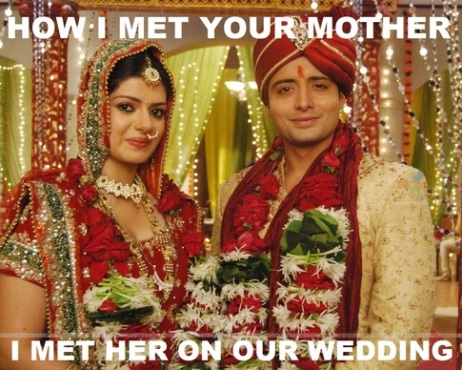
\includegraphics[width=2.0449in,height=1.6335in]{figures/chap2/chapitre2-img6.jpg}
    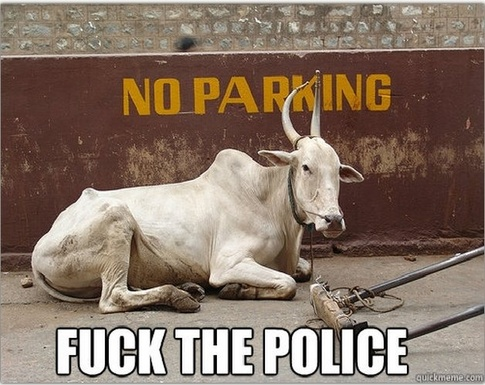
\includegraphics[width=2.078in,height=1.6449in]{figures/chap2/chapitre2-img7.jpg}
    \caption{Exemples de réponses à la question \textit{"What are some quintessential Indian memes ?"} D'après \url{http://www.quora.com/India/What-are-some-quintessential-Indian-memes}, Consulté le 12/08/2013 à 0 :41 GMT+8 }
    \label{fig:quora-india}
\end{figure}


Avec plusieurs centaines d{\textquoteright}images postées par des
utilisateurs majoritairement indiens\textsuperscript{7}, nous pouvons
constater plusieurs choses : 

\begin{itemize}
\item
\textbf{Langue}: à part trois réponses, la totalité des réponses sont en anglais. Cela peut s’expliquer par le fait que l’anglais est une langue de communication majoritaire en Inde, et également par le fait que le site Quora.com n’accepte habituellement que des réponses en anglais.
\item
\textbf{Forme}: à l’exception de quatre réponses, les mèmes revêtent tous la forme « classique » : photo retouchée et légendé par un texte en anglais aux lettres blanches sur fond ou détour noir.

\item
\textbf{Humour}: la plupart des réponses sont de nature comique.
\item
\textbf{Récurrence}: certaines images sont très récurrentes et si les légendes diffèrent, le sens reste le même.
\item
\textbf{Thématiques diverses}: de nombreux messages traitent de la vie de famille (parents, mariage), de loisirs (cricket), de la vie quotidienne (achats, école , etc.) et un peu de politique.
\end{itemize}

L{\textquoteright}image la plus citée représente la figure
d{\textquoteright}un père autoritaire :

\begin{figure}

    \subfloat[\textit{"High Expectations Indian Father"}]{
        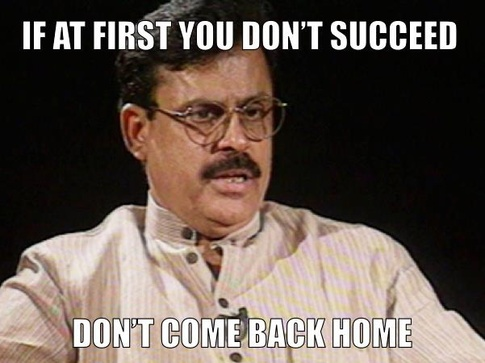
\includegraphics[width=2.0449in,height=1.5in]{figures/chap2/chapitre2-img8.jpg}
        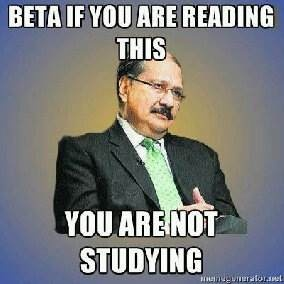
\includegraphics[width=1.5335in,height=1.5in]{figures/chap2/chapitre2-img9.jpg}
        
\includegraphics[width=1.8224in,height=1.5in]{figures/chap2/chapitre2-img10.jpg}
        \label{fig:severe-indian-dad}
    }
    \newline
    \subfloat[\textit{"High Expectations Asian Father"}]{
        \label{fig:severe-chinese-dad}
        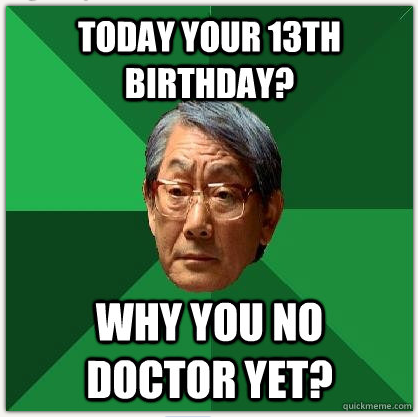
\includegraphics[width=1.9335in,height=1.9in]{figures/chap2/chapitre2-img11.png}
        
\includegraphics[width=1.9004in,height=1.9in]{figures/chap2/chapitre2-img12.jpg}
        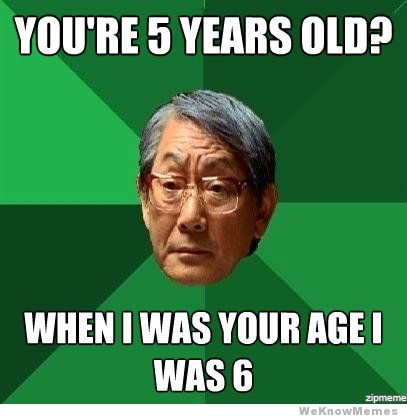
\includegraphics[width=1.8449in,height=1.9in]{figures/chap2/chapitre2-img13.jpg}
    }
    \caption[Mème "High Expectations Asian Father" d'après Quora.com]{Exemples du mème \textit{"High Expectations Asian Father"} D{\textquoteright}après {\textquotedblleft}\textit{What are the funniest High Expectations Asian Father meme images?{\textquotedblright}} sur Quora.com \url{http://www.quora.com/Memes/What-are-the-funniest-High-Expectations-Asian-Father-meme-images}, Consulté le 12/08/2013 à 10:56}
\end{figure}

La définition des mèmes faites par Blackmore ne correspond pas nécessairement à ce que nous observons ici. L{\textquoteright}unité formelle de l{\textquoteright}ensemble de ces mèmes (image avec des caractères blancs cerclés de noirs) propose une définition bien plus restreinte. Néanmoins, nous pouvons comprendre qu{\textquoteright}il s{\textquoteright}agit bien de la manifestation d{\textquoteright}une culture particulière. L{\textquoteright}image d{\textquoteright}une vache assise devant un sigle \textit{{\textquotedblleft}Fuck The Police{\textquotedblright} }serait en effet un absolu non-sens sans la référence à l{\textquoteright}Inde o\`u les vaches sont sacrées et jouissent de droits particuliers que même la police ne peut entraver. Ainsi, il existe bel et bien des pré-requis pour comprendre ou actualiser un mème. Les plus évidents sont :

\begin{itemize}
    \item \textbf{L’accès et l’usage de la bonne technologie}: Il est nécessaire pour un utilisateur de posséder et de savoir utiliser la technologie par laquelle le mème est diffusé.
    \item \textbf{La langue}: Le message possède une légende donc l’utilisateur doit pouvoir la lire et la comprendre.
    \item \textbf{Les implicites} : L’utilisateur doit posséder le socle de références communes et d’implicites qui sont impératifs pour pouvoir comprendre le message. 
\end{itemize}

Nous observons ici de très larges et vagues groupes ({\guillemotleft}~\textit{indiens}~{\guillemotright}, {\guillemotleft}~\textit{asiatiques}~{\guillemotright}{\dots}) sans pouvoir vraiment comprendre dans le détail ce qui peut réellement constituer des éléments communs. Les travaux sur la formation des {\textquotedblleft}communautés{\textquotedblright} en ligne ont montré comment la circulation des objets digitaux peut posséder une fonction de catharsis pour des groupes plus réduits \citep{Steyer2006}. Néanmoins, on voit bien qu{\textquoteright}ici l{\textquoteright}appartenance pré-existe puisque le mème nécessite de nombreux pré-requis pour le comprendre. Le langage et son expressivité par l{\textquoteright}humour sont notamment des contraintes incompressibles pour l{\textquoteright}actualisation de ce mème par un individu. Néanmoins nous pouvons voir dans ce cas particulier que le mème participe à l{\textquoteright}affirmation de l{\textquoteright}existence du groupe, avec la figure redondante de caractéristiques communes du père, affirmant par la dérision une forme de paternité commune aux membres de ce groupe. D{\textquoteright}autres mèmes ne nécessitent pas tant de références, ce qui contribue largement à leurs diffusions. La vidéo du clip musical \textit{Gangnam Style} du chanteur Psy a notamment atteint des records inégalés en termes de diffusion\footnote{ Première vidéo à avoir officiellement dépassée le milliard de vues sur Youtube. 1,733,769,243 vues, consulté le 13/08/2013 à 09 :35 GMT+8 \url{http://www.youtube.com/watch?v=9bZkp7q19f0}} gr\^ace à une très vaste campagne télévisuelle et sur internet. La diminution des implicites et la standardisation de l{\textquoteright}écriture utilisée a sans doute contribué la diffusion, avec un langage du corps quasi universel, le pas de danse. Formellement, il s{\textquoteright}agit d{\textquoteright}un vidéo clip très classique dont la structure et le montage sont largement familiers du public. Les attributs des personnages du clip sont également de grands classiques du vidéo clip commercial : voitures, belles filles et bijoux en or. La présence d{\textquoteright}un quartier spécifique de Séoul en Corée du Sud agit ici comme un attribut du contenu mais aucune des références ne nécessite de préalable linguistique particulier. De plus, les mystères de la musique et de la scénographie agissent bien évidemment au delà de toute analyse formelle pour faire de ce hit un des mèmes Internet les plus connus dans le monde. 
Les méméticiens disposent classiquement de deux procédes pour
analyser la diffusion des mèmes: 

\begin{itemize}
\item
\textbf{La contamination~\newline
}Le mème se déplace à la manière d{\textquoteright}un virus, en contaminant les sujets les plus susceptibles de l{\textquoteright}être lors d{\textquoteright}une phase d{\textquoteright}exposition. L{\textquoteright}exemple le plus classique pour ce modèle est la diffusion des croyances religieuses
qui agirait par contagion \citep{Dennett2006}
\item
\textbf{La réplication~\newline
L}es activités culturelles humaines procèdent de l{\textquoteright}imitation, notamment au travers de phases cruciales d{\textquoteright}apprentissage. Ainsi, les mèmes existent et se diffusent dans toutes activités nécessitant une imitation : \textit{{\textquotedblleft}} \textit{If we define memes as transmitted by imitation then whatever is passed on by this copying process is a meme.{\textquotedblright} }\citep{Blackmore2006}. 
\end{itemize}

Le modèle épidémique de diffusion vient appuyer la vision éthologique du mème. Adaptée de la virologie, les {\guillemotleft}~sujets à risque~{\guillemotright} seraient plus à même d{\textquoteright}être {\guillemotleft}~contaminés~{\guillemotright} par une {\guillemotleft}~exposition~{\guillemotright} suffisamment longue à tel ou tel mème \citep{Wang2011}. Blackmore définit néanmoins trois phases indispensables pour reconna\^itre un mème comme tel:  

\begin{quote}
Memes fulfill the role of replicator because they exhibit all three of the necessary conditions; that is, \textit{heredity} (the form and details of the behavior are copied), \textit{variation} (they are copied with errors, embellishments or other variations), and \textit{selection} (only some behaviors are
successfully copied). \citep{Blackmore2006}
\end{quote}

Les trois aspects sont indissociables et forment selon Blackmore un {\textquotedblleft}\textit{véritable processus évolutioniste{\textquotedblright} }\citep{Blackmore2006}. La définition quasi tautologique du mème ({\guillemotleft}~\textit{Whatever is passed on{\guillemotright}}) montre bien comment le mème en tant que concept est considéré chez Blackmore non pas comme un phénomène mais plutôt comme un objet en-soi. La définition du mème en tant qu{\textquoteright}objet autonome se heurte dès l{\textquoteright}abord au risque de devenir un pur artefact de l{\textquoteright}observation, n{\textquoteright}existant que dans l{\textquoteright}esprit de l{\textquoteright}observant. Alors que Dawkins met en garde non sans humour que son livre \textit{The Selfish Gene} \textit{{\textquotedblleft}devrait être lu presque comme s{\textquoteright}il était de la science-fiction{\textquotedblright} }\citep{Dawkins1989}, la faiblesse des modèles de diffusion des mèmes vu comme un réplicateur ou comme un virus ne recouvre que partiellement la réalité observée empiriquement pour les mèmes Internet. Ainsi, l{\textquoteright}appartenance des individus à tel ou tel groupe pré-existe au mème. Dans son appropriation se joue davantage l{\textquoteright}expression d{\textquoteright}un sentiment d{\textquoteright}appartenance qu{\textquoteright}une contamination qui nierait les termes de sa volonté individuelle pour y substituer l{\textquoteright}individu comme sujet du mème.  


\section[Textualité des mèmes et formes d{\textquoteright}énonciations numériques]{Textualité des mèmes et formes d{\textquoteright}énonciations numériques}

\subsection[Le mème comme figure rhétorique de l{\textquoteright}écriture intertextuelle]{Le mème comme figure rhétorique de l{\textquoteright}écriture intertextuelle}

 
Nous t\^acherons donc ici de définir le mème comme une série d{\textquoteright}actes \textit{d{\textquoteright}énonciation }qui contribuent à l{\textquoteright}existence et la reconnaissance mutuelles d{\textquoteright}individus comme groupe, à l{\textquoteright}opposé d{\textquoteright}un élément de sémantique pure qui serait constitutif d{\textquoteright}une hypothétique culture commune. Les partages, commentaires, réappropriations puis transformations des \textit{mèmes Internet }nous serviront de supports pour comprendre les \textit{actes d{\textquoteright}énonciation. }Ces courts messages faits de texte, image ou vidéo sont en quelque sorte les voix, répétitions, annonances et redites d{\textquoteright}une foule d{\textquoteright}individus et de groupes qui habitent la Toile. Au-delà de l{\textquoteright}idée d{\textquoteright}un {\textquotedblleft}objet{\textquotedblright} numérique qui réifierait les actions en une substance figée, nous nommons \textit{énonciation} le moment d{\textquoteright}existence observable o\`u se manifeste un mème. Comme pour les émoticones, les pratiques actuelles de l{\textquoteright}écriture en ligne des mèmes Internet sont à envisager comme des formes renouvelées d{\textquoteright}oralité. Email, chat ou réseaux sociaux, ces discussions font partie d{\textquoteright}une \textit{{\textquotedblleft}oralité seconde{\textquotedblright} }\citep{Ong1988} constituante des technologies de l{\textquoteright}écrit à l{\textquoteright}ère du numérique. Contrairement à l{\textquoteright}oralité première des illettrés, cette oralité seconde est structurée par l{\textquoteright}usage des technologies et notamment les structures formelles de l{\textquoteright}écriture pour le média :  

\begin{quote}
Telephone, radio, television and the various kind of sound tape, electronic technology has brought us into the age of {\textquoteleft}secondary orality{\textquoteright}. This new orality has striking resemblance to the old in its participatory mystique, its fostering of a communal sense, its concentration on the present moment, and even its use of formulas. But it is essentially a more deliberate and self-conscious orality, based permanently on the use of writing and print, which are essential for the manufacture and operation of the equipment and for it use as well. 
\citep{Ong1988}
\end{quote}

L{\textquoteright}hypothèse de Ong est ici que l{\textquoteright}oralité des écritures numériques est une forme manufacturée de l{\textquoteright}expression orale, à laquelle préside la production (industrielle) des technologies. Les services de réseaux sociaux en ligne confirment l{\textquoteright}hypothèse première de Ong puisque \textit{Sina Weibo }ou \textit{Twitter }contraint l{\textquoteright}écriture à une longueur maximum de 140 caractères. Néanmoins, l{\textquoteright}oralité du mème Internet et plus généralement des écritures numériques ne procède pas seulement de cette écriture conditionnée mais également de la mise en relation des textes : l{\textquoteright}intertextualité. Là o\`u pour Ong l{\textquoteright}industrie médiatique vient contraindre l{\textquoteright}écriture pour la réifier en produit industriel simulant l{\textquoteright}oral, l{\textquoteright}intertextualité vient subvertir ces limites imposées en renvoyant le lecteur à la page suivante.  

En effet, le langage des nouveaux médias ne se contente pas de proposer des nouvelles opérations d{\textquoteright}interactions et de navigations mais s{\textquoteright}inscrit également dans de nouveaux modes de lecture et de narration \citep{Manovich2001}. Une des grandes difficultés pour l{\textquoteright}analyse textuelle et narrative dans le cadre des nouveaux médias est de comprendre o\`u commence et o\`u se termine la narration. La structure éminemment relationnelle du discours narratif en ligne et son intertextualité en font un objet mal défini, que ses auteurs n{\textquoteright}ont pas signé d{\textquoteright}un point final. L{\textquoteright}étude des discursivités hypertextuelles s{\textquoteright}apparenterait donc davantage à l{\textquoteright}étude des formes dans les contes et légendes qu{\textquoteright}aux études herméneutiques classiques sur des textes finis \citep{Clement1995}. Comme le note Lévi-Strauss dans son travail sur Propp, même si les contes possèdent souvent une structure similaire, leur étude en tant qu{\textquoteright}élément culturel n{\textquoteright}est révélatrice que dans un contexte précis et incarné. Il est inutile de vouloir extraire une supposée intention culturelle du texte car on se doit de le comprendre lors de son énonciation, sur la place d{\textquoteright}un marché au Maroc avec les conteurs de Ben Jelloun ou au pied du lit d{\textquoteright}un jeune Européen avec les histoires compilées par les frères Grimm. Héritant à la fois des pratiques culturelles et folkloriques anciennes tout en se renouvelant sous les nouvelles contraintes de la technologie \citep{Barber2008}, le mème est lui aussi à comprendre dans son contexte d{\textquoteright}énonciation. De récents travaux travaillent à comparer les modes de diffusion des mèmes avec ceux des traditions folkloriques \citep{Seta2014}. En considérant les mèmes Internet comme un {\textquotedblleft}\textit{folklore numérique{\textquotedblright}, }on comprend mieux la nature presque auto-référentielle de la relation entre le mème et la culture qui le voit na\^itre. La transmission d{\textquoteright}éléments particuliers dans la discursivité du mème en fait une figure rhétorique d{\textquoteright}énonciation de sa propre origine. Habituellement définie comme \textit{{\guillemotleft}~une forme typique de relation non linguistique entre des éléments discursifs.~{\guillemotright}}\footnote{ \textit{Les figures de rhétorique}, Laurent Jenny, Université de Genève, 2003}\textit{, }la figure rhétorique se produit dans l{\textquoteright}intertextualité des redites et commentaires qui réaffirme dans le mème l{\textquoteright}existence d{\textquoteright}un groupe qui le constitue.  

Le large pouvoir fédérateur de certains mèmes fascine. Diffusés très largement, \ on se plait à imaginer comment ils peuvent réunir en leur sein des groupes et individus distants, auparavant inconnus et étrangers. L{\textquoteright}importance croissante d{\textquoteright}Internet dans l{\textquoteright}émergence de groupes d{\textquoteright}intérêts et d{\textquoteright}activités voit les études sur la formation de communautés en ligne fleurir. Néanmoins, il nous semble important de se questionner sur la nature des relations créée lors des discussions partagées en ligne. Est-ce bien là le fait d{\textquoteright}une réelle rencontre comme le croient les plus enthousiastes? Ou au contraire est-ce le produit d{\textquoteright}une machine médiatique et décérébrante qui produit du lien sans engendrer de rencontres comme le pensent les plus pessimistes? Cette vaste question est sans doute un des enjeux centraux des questionnements autour de l{\textquoteright}Internet, notamment pour le management et les sciences de gestion. Si l{\textquoteright}énonciation est une pratique structurante pour un individu ({\textquotedblleft}je suis{\textquotedblright}), elle peut l{\textquoteright}être également pour un groupe ({\textquotedblleft}nous sommes{\textquotedblright}). Dans la perspective empirique o\`u nous nous situons, il nous faut tout d{\textquoteright}abord interroger les pratiques du langage pour mieux comprendre comment les discursivités d{\textquoteright}un mème peuvent agir sur les groupes. Le mème en tant considéré comme un acte d{\textquoteright}énonciation se caractérise non seulement par sa manifestation langagière, mais également par l{\textquoteright}intention qu{\textquoteright}il contient. Dans le cadre des réseaux sociaux, nous ne disposons que de très peu d{\textquoteright}éléments sur l{\textquoteright}intention car les données disponibles sur les réseaux sociaux sont par définition le résultat d{\textquoteright}actions passés (écriture, clics, etc.).\textit{ }Nous devons donc développer un modèle à la fois conceptuel et pratique pour nous permettre d{\textquoteright}étudier ces phénomènes d{\textquoteright}énonciation dans le cas particulier des mèmes Internet. Wittgenstein dans ses \textit{Recherches Philosophiques }défend une analyse pragmatique du langage en écrivant : \textit{{\textquotedblleft}Don{\textquoteright}t ask for the meaning, ask for the use.{\textquotedblright}} \citep{Wittgenstein2004}. Ainsi, il s{\textquoteright}agit de comprendre les jeux langagiers non pas comme un champ linguistique mais comme un ensemble d{\textquoteright}actes qui font sens en contexte et possèdent une intention. 

\begin{quote}
{\textquotedblleft}Expressions have meanings even when they are not being used, but it is only in using expressions that a person means something.{\textquotedblright} \citep{Bach1994}
\end{quote}

Austin dans ses lectures sur William James met au centre du langage sa dimension pragmatique et propose de comprendre comment on \textit{{\guillemotleft}~fait des choses avec les mots~{\guillemotright}} \citep{Austin1975}. Ses le\c{c}ons présentent une manière nouvelle de catégoriser les différents actes d{\textquoteright}énonciation et montrent la grande diversité des éléments non-linguistique présents dans ces actes. Austin introduit le concept de \textit{performativité }pour nommer le processus qui permet de construire par le langage une réalité extérieure au langage. Les mots ne nomment pas seulement les choses mais peuvent également les faire changer, voire les fabriquer. Austin s{\textquoteright}intéresse donc aux énoncés selon leurs \textit{sens}, leurs intentions (la \textit{force}) ou leurs \textit{effets}. Le concept de \textit{performativité }a depuis continué son chemin tant en linguistique qu{\textquoteright}en sciences sociales, et plus récemment dans des champs aussi divers que le management ou l{\textquoteright}étude du discours scientifique et des pratiques légales \citep{Denis2006}. Les économistes également ont beaucoup discuté de la performativité des discours économiques sur l{\textquoteright}économie réelle \citep{Mackenzie2006}. Les \textit{cultural studies,} et plus précisément les \textit{gender studies }ont aussi fait un large usage de ce concept pour exprimer l{\textquoteright}influence de la matérialité des mots sur les comportements humains \citep{Butler1993}.  

\begin{quote}
{\guillemotleft}~Pour qu{\textquoteright}ils deviennent de {\guillemotleft} véritables {\guillemotright} performatifs, les faits, les théories ou les formules doivent circuler dans des cha\^ines de traduction qui consolident l{\textquoteright}assemblage des entités qui le composent et leur permet d{\textquoteright}acquérir le statut de {\guillemotleft} matters of fact {\guillemotright} ({\dots}). C{\textquoteright}est lorsqu{\textquoteright}ils arrivent à durer, c{\textquoteright}est-à-dire à s{\textquoteright}inscrire dans le monde (par l{\textquoteright}intermédiaire d{\textquoteright}objets, de textes, de dispositifs techniques complexes) que leur performativité s{\textquoteright}accomplit.~{\guillemotright} \citep{Denis2006}
\end{quote}

Les actes d{\textquoteright}énonciation répétés modèlent donc le corps des personnes et de la société, y \textit{laissant }durablement leurs marques. Les énoncés actualisent les discours des groupes sociaux sur eux-mêmes \citep{Butler1993} et ce caractère performatif est constitutif de l{\textquoteright}énonciation. Les énoncés collectifs que sont les mèmes Internet possèdent également cette dimension performative qui actualise le discours de certains groupes en réalités tangibles. La circulation et la structuration de ces mèmes vient structurer le milieu numérique et peut ainsi influer sur la définition de groupes sociaux et des rapports qu{\textquoteright}ils entretiennent. Une image ou un mot d{\textquoteright}un mème ne peut néanmoins devenir commune sans le préalable permettant de dénouer l{\textquoteright}implicite de l{\textquoteright}énoncé, faisant de l{\textquoteright}énonciation un accroissement de proximité dans l{\textquoteright}expérience dans le moment. Blackmore évoque en termes évolutionnistes le {\textquotedblleft}potentiel transformatif{\textquotedblright} du mème, avec ce qu{\textquoteright}elle nomme la \textit{variation} puis la \textit{sélection. }Ici ce sont les actes d{\textquoteright}\textit{énonciation} qui forment une praxis du mème. Pour nous, le mème n{\textquoteright}est pas un méta-symbole en évolution mais un réseau de praxis culturelles constitué de multiples d{\textquoteright}actes d{\textquoteright}énonciation. Ainsi, le mème ne peut être simplement {\guillemotleft}~copiée~{\guillemotright} mais a besoin d{\textquoteright}être acté pour exister. Dans la définition du mème de Blackmore comme dans le cas des réseaux sociaux, nous observons que l{\textquoteright}énonciation d{\textquoteright}un mème procède d{\textquoteright}une variation parfois nulle, parfois minimale, parfois importante de sa forme d{\textquoteright}origine. Cette déformation due à l{\textquoteright}énonciation est le propre de la fonction d{\textquoteright}apprentissage, notamment langagier. Le caractère performatif du mème devient visible dans l{\textquoteright}usage approprié de la variation qui en est fait. 

Le succès de l{\textquoteright}intention de l{\textquoteright}énoncé est visible dans son imitation, avec comme garantie l{\textquoteright}erreur ou la variation. Platon dans \textit{La République} puis par la suite Aristote dans sa \textit{Poétique,} s{\textquoteright}interroge sur la notion de \textit{mimesis} définie comme les formes d{\textquoteright}imitation qui permettent soit de reproduire, soit de styliser la nature. Pour Aristote, le but singulier de la mimesis est de mettre à jour la dimension empathique cachée de la nature, de la styliser pour y révéler le continuum de l{\textquoteright}expérience propre à tous les êtres. Plus l{\textquoteright}artiste s{\textquoteright}approche de la nature en se dirigeant vers une imitation {\guillemotleft}~véritable{\guillemotright}, plus il s{\textquoteright}éloigne de la réalité de la nature. L{\textquoteright}importance d{\textquoteright}une approche rhétorique comme par exemple la stylisation devient le véritable moyen d{\textquoteright}accès à la signification profonde des choses. Freud réutilisera le concept de \textit{mimesis} pour décrire l{\textquoteright}énonciation du sens d{\textquoteright}un évènement traumatique passé dans la vie d{\textquoteright}un individu au travers d{\textquoteright}activités créatives (art, parole, rêves etc.). Dans la continuité d{\textquoteright}Aristote, Freud comprend le rêve comme une \textit{mimesis} du passé et du réel, révélant au sujet un objet symbolique enfoui. Peut-être est-il possible de considérer le mème Internet comme une mimesis des groupes sociaux et médiatiques qui le produisent. Les processus de symbolisation et de stylisation jouent en effet un rôle déterminant dans sa diffusion. Acte d{\textquoteright}énonciation, le mème agit alors comme une \textit{mimesis} des activités et états d{\textquoteright}\^ame de groupes d{\textquoteright}individus qui l{\textquoteright}énoncent. S{\textquoteright}il est possible de le revivre plusieurs fois, il prendra peut-être à chaque fois un sens différents. Comme le rêve freudien qui est une manifestation biologique de la mémoire inconsciente se produisant durant le sommeil, le mème se manifeste sous des formes visibles symboliques incarnées, \textit{mimesis} particulière du groupe des individus qui l{\textquoteright}énoncent. 


\subsection[Typologie des mèmes Internet]{Typologie des mèmes Internet}

En nous appuyant sur la littérature concernant les figures
rhétoriques, nous pourrions chercher à définir plus
précisément une typologie des mèmes fondée sur les formes du
discours. En grec ancien, le topo\"i défini à la fois un lieu ou un
endroit mais également un ensemble de formes rhétoriques utilisant
des motifs particuliers lors de l{\textquoteright}argumentaire afin de
persuader lors de joutes oratoires. En littérature comme en
mathématiques, le terme de \textit{topos }définit également un
ensemble de catégories ouvertes mais connues,
\textit{{\textquotedblleft}un protocole de description des univers
possibles{\textquotedblright} }\citep{Badiou2006}. Le mème peut donc
être compris comme un \textit{lieu commun, }idée
{\textquotedblleft}re\c{c}ue{\textquotedblright} utilisant des
situations ou des images communes et stéréotypées pour opèrer
une transformation sémantique en jouant sur la répétition
d'éléments (les sèmes du discours). En
rhétorique, l{\textquoteright}usage du topos a pour objectif de
contribuer à la persuasion de l{\textquoteright}auditeur par la
mobilisation subtile d{\textquoteright}éléments de culture commune.
Tout l{\textquoteright}art du rhéteur consiste à trouver un moyen
subtile d{\textquoteright}actualiser un lieu commun en une situation
unique propre au contexte pour convaincre. Dans le discours, il prend
bien souvent la forme de l{\textquoteright}anecdote que la rumeur se
charge de diffuser, sa diffusion étant d{\textquoteright}autant plus
efficace qu{\textquoteright}il possède un caractère amusant ou
railleur \citep{Flaubert1997} Concevoir le mème comme une forme de
pratique rhétorique semblable au lieu commun nous permet de resituer
le phénomène des mèmes Internet dans la continuité historique
des pratiques de l{\textquoteright}écriture et de
l{\textquoteright}énonciation rhétorique, ainsi que de ses
modèles d{\textquoteright}analyse socio-textuelle et littéraire
\citep{Plantin1993}. Ainsi, nous pouvons aborder la lecture des mèmes
Internet sous le jour de leur existence aussi bien formelle (textuelle)
que rhétorique (comme actes d{\textquoteright}énonciations et de
persuasion). Les mèmes tout comme les lieux communs se donnent à
voir d{\textquoteright}abord sous la forme de paradoxes, qui
deviendront eux-mêmes des lieux communs.
L{\textquoteright}originalité d{\textquoteright}un lieu commun en
devenir se définit dans une tension constante entre imitation et
nouveauté, subversion et actualisation de formes canoniques :
\textit{{\textquotedblleft}dialogue de l'horizon
d'attente et de l'écart esthétique, c'est-à-dire le jeu du classique et du moderne, la tension entre le même et l'autre qui existe, dans tout texte et dans toute lecture, entre le plaisir et la jouissance, pour reprendre les mots de Barthes}. \citep{Compagnon1997}

L{\textquoteright}approche des mèmes renouvelée par la nature
intertextuelle du langage multimédia montre des caractéristiques
 d{\textquoteright}après une centaine de mèmes parmi les plus
largement diffusés d{\textquoteright}Internet : 

\begin{enumerate}
\item {\color{black}
\textbf{Humour~}: Le mème doit posséder une dimension comique et
accrocheuse}
\item {\color{black}
\textbf{Intertextualité} : Le mème met en jeu un ou des renvois à
d{\textquoteright}autres éléments culturels ou textuels, souvent
implicites.}
\item {\color{black}
\textbf{Juxtaposition atypique} : Les éléments visuels ou
sémantiques mis en jeu dans le mème ne possèdent pas de
corrélations apparentes et c{\textquoteright}est la mise en relation
de plusieurs objets improbables qui en fait un objet intéressant.}
\end{enumerate}
L{\textquoteright}étude en question nous offre un début de
critères mais porte seulement sur un type précis de mèmes à
caractère plutôt comique, ignorant les discussions plus
sérieuses, d{\textquoteright}ordre politique notamment. La forme
particulière de juxtaposition atypique observée par les auteurs
serait en rhétorique une {\textquotedblleft}\textit{métaphore in
praesentia{\textquotedblright} }décrite comme une
\textit{{\guillemotleft}~figure de rapprochement analogique entre deux
représentations co-présentes~{\guillemotright}} \citep{Jenny2012}. Nous
nous trouvons donc en présence d{\textquoteright}une forme
particulière de mème seulement. Si l{\textquoteright}humour sous
toutes ces formes (blague, sarcasme, ironie, etc.) est un élément
très répandu qui favorise la circulation des contenus en ligne, il
nous semble néanmoins un peu réducteur de se limiter à cette
définition. De nombreux mèmes Internet existent non pas gr\^ace à
l{\textquoteright}humour mais gr\^ace au \textit{pathos}
qu{\textquoteright}ils dégagent. Le mème \textit{Kony2012, }un des
plus diffusés de l{\textquoteright}histoire
d{\textquoteright}Internet, présentait le militaire Ugandais Joseph
Kony dans une vidéo faite d{\textquoteright}images de guerre et
d{\textquoteright}enfants en pleurs\footnote{ \textit{KONY2012: See How Invisible Networks Helped a Campaign Capture the World's Attention}, \textit{Social Flow}, \url{http://alturl.com/zniry} consulté le 28 Février 2014 GMT+1}.
Ainsi, on peut dire que les mèmes Internet utilisent les formes
classiques de la rhétorique adaptées au langage médiatique moderne
teinté d{\textquoteright}humour ou de sensationnalisme. En se
saisissant du monde social et politique, les mèmes Internet
produisent d{\textquoteright}intéressants discours sur les faits
qu{\textquoteright}ils relatent - et sur la technologie qui les
produit. Alors que les révolutions du Printemps Arabe avaient
notamment soulevé l{\textquoteright}espoir d{\textquoteright}un monde
meilleur par l{\textquoteright}usage des réseaux sociaux pour
instaurer la démocratie \citep{Lotan2011}, la communication
instantanée via ces mêmes réseaux sociaux devenait quelques
semaines plus tard une des causes majeures de la flambée de violence
durant une série d{\textquoteright}émeutes à Londres (Casilli \&
Tubaro, 2011). Les différentes intentions des discursivités et
actes d{\textquoteright}énonciation à l{\textquoteright}{\oe}uvre
dans un mème peuvent donc nous aider à dresser une typologie des
mèmes. Une typologie des mèmes ne peut être considérée comme
exclusive et les glissements sémantiques et symboliques qui peuvent
s{\textquoteright}opérer nous obligent à considérer une
catégorisation non-exclusive. En nous appuyant sur différents
exemples et sur la littérature, nous dressons une première
ébauche de typologie des mèmes Internet qui sera ensuite
approfondie par l{\textquoteright}étude empirique des données le
c{\oe}ur de notre étude. Pour les exemples, nous essaierons de donner
les références et implicites indispensables permettant de
comprendre le mème dans son intertextualité.

\begin{table}
    \centering
    \begin{tabulary}{\textwidth}{ R | C}
    \textbf{Objectifs du mème}  & \textbf{Exemples célèbres et références} \\[0.2ex]
    \hline \\ [-1.5ex]
    Absurdiste, humour &  LOLCats, Tumblr \citep{Bauckhage2011} \\[0.3ex]
    \hline \\ [-1.5ex]
    Actualité, satire, commentaire social  & CaoNiMa \citep{Mina2012}, Cute Cat Theory \citep{Zuckerman2008} \\[0.3ex]
    \hline \\ [-1.5ex]
    Publicité, marketing viral & Gangnam Style \citep{Bolsover2013}, Memetic Marketing \citep{Flor2000} \\[0.3ex]
    \hline \\ [-1.5ex]
    Marketing politique, soutien, pétition & Obama Ohio Campaign \citep{Walker2012}, Pétitions en ligne (Adamic al.,2013) \\[0.3ex]
    \hline \\ [-1.5ex]
    Fan clubs, adoration  &  Fan-fiction , Machinima, etc. \\[0.3ex]
    \hline \\ [-1.5ex]
    Hoax, spam & Email spam, « Nigerian scam » \\[0.3ex]
    \end{tabulary}

\caption[Typologie des mèmes]{Les différents type de mèmes Internet observables - tableau réalisé d{\textquoteright}après la littérature indiquée}
\label{fig:typologie-memes}

\end{table}


Cette typologie nous permet de poser un premier regard sur des catégories non-exclusives constituant le paysage des mèmes Internet, inspirés d{\textquoteright}exemples et de la littérature existante. Nous pouvons d{\textquoteright}ores et déjà noter que l{\textquoteright}ensemble de ces différentes pratiques pré-existent à l{\textquoteright}Internet et sont souvent la reconduction sous une forme numérique de discursivités pré-existantes (penser à la publicité, la propagande politique ou même les rumeurs). La forme et l{\textquoteright}échelle de la diffusion sont néanmoins des différences importantes ainsi bien s\^ur que \ les situations d{\textquoteright}énonciation (dans une file d{\textquoteright}attente ou devant son ordinateur). 

Voici donc cette typologie plus en détails et illustrée d{\textquoteright}exemples. 


\begin{description}

\item[Absurdiste, humour]
\hfill \\
De nombreux mèmes Internet parmi ceux que nous avons présentés dans la première partie de ce chapitre viennent se classer dans cette catégorie. Connaissant parfois des succès planétaire, un des exemples les plus caractéristiques est celui des {\textquotedblleft}LOLcats{\textquotedblright}, ces vidéos ou images de chats illustrés de citations et autres accessoires comiques. Omniprésent sur la Toile, l{\textquoteright}immense répertoire de photos et de vidéos comiques de chats dans différentes situations (jouant du piano, sautant dans des bo\^ites en cartons, etc.) constitue un des plus visionnés de l{\textquoteright}Internet \citep{Bauckhage2011}. 

\item[Actualité, satire, commentaire social]
\hfill \\
En regroupant ces trois catégories, nous souhaitons considérer la pratique ancienne des discussions politiques ou polémiques autour de faits divers ou d{\textquoteright}actualités que l{\textquoteright}Internet vient aujourd{\textquoteright}hui renouveler dans la forme. Nous avons vu précedemment avec les {\textquotedblleft}crabes de rivières{\textquotedblright} (voir 1.2.2.) \textcolor[rgb]{0.0,0.0,0.039215688}{comment la satire politique en Chine se manifestait bien souvent sous la forme de mèmes Internet. Par les voies de l{\textquoteright}Internet, }de nombreux faits divers sont devenus en Chine des affaires d{\textquoteright}état, influen\c{c}ant le jeu politique et offrant un nouveau canal de diffusion pour les pratique subversives. Connu pour son {\oe}uvre artistique, l{\textquoteright}artiste chinois Ai Weiwei est une des figures célèbres de l{\textquoteright}Internet chinois. Utilisant abondamment blog et microblog, son travail artistique depuis plusieurs années a pris la tournure d{\textquoteright}un bras de fer médiatique avec le gouvernement sur les grandes questions sociétales de la Chine d{\textquoteright}aujourd{\textquoteright}hui. Son père, poète célèbre du régime communiste sous Mao fut déchu durant la révolution Culturelle, transmettant à son fils à la fois un go\^ut pour les arts et une violente amertume pour le pouvoir en place à Pékin. Critiquant ouvertement la corruption des officiels et de la police, Ai Weiwei a vu régulièrement ses comptes Internet de blog et microblog fermés, notamment par le service Sina Weibo. Sur Twitter néanmoins, il jouit d{\textquoteright}une grande popularité avec près de de 200.000 \textit{{\textquotedblleft}followers{\textquotedblright}} pour son compte officiel @aiww. Au fil de son blog relatant ses nombreux déboires avec le gouvernement, on croise bien souvent une figure mythologique né de la toile chinoise, le \textit{caonima}.  

\begin{figure}
    \centering
    
    \subfloat[Une image de la vidéo originale représentant le \textit{caonima}.]{
        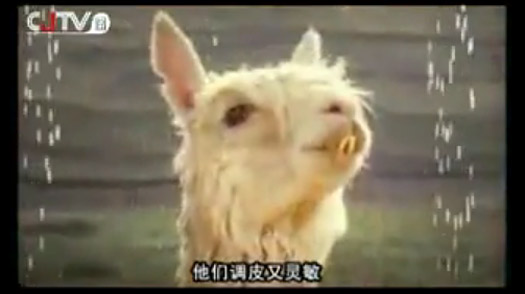
\includegraphics[width=3.7894in,height=2.1224in]{figures/chap2/chapitre2-img14.jpg}
    }
    \subfloat[Un caractère chinois composé spécialement par les internautes pour signifier cet animal mythique]{ 
        
\includegraphics[width=2.0559in,height=2.0559in]{figures/chap2/chapitre2-img15.jpg}
    }
    \caption[\textit{Caonima}: un animal mythique du web chinois]{\textit{Caonima}: un animal mythique du web chinois, d{\textquoteright}après le \textit{Grass-Mud Horse Lexicon Classics}publié par \textit{China Digital Times }(2013)}
    \label{fig:caonima}

\end{figure}

Luttant contres les crabes de rivière, le \textit{caonima }symbolise la lutte contre la censure pour un Internet libre. Apparu pour la première fois dans une vidéo virale\footnote{ \textit{Song of the Grass-Mud Horse (Cao Ni Ma), }Youtube \ \url{https://www.youtube.com/watch?v=wKx1aenJK08}, consulté le 28 Février 22:08\par }, le \textit{caonima} est un animal de la famille des camélidés (l{\textquoteright}alpaga) courant fièrement dans les prés sur une petite musique de dessin animé aux paroles entièrement réécrites pour l{\textquoteright}occasion. Littéralement {\textquotedblleft}cheval d{\textquoteright}herbe et de boue{\textquotedblright}, le mot {\textquotedblleft}caonima{\textquotedblright} [FF08?][8349?][6CE5?][9A6C?][FF09?]cache en fait un double sens puisque son homophone ([64CD?][4F60?][5988?]) est une grossière interjection à l{\textquoteright}intention des génitrices des censeurs de Pékin. Devenu aujourd{\textquoteright}hui une véritable icône anti-censure, il n{\textquoteright}est pas rare de le croiser sur un tee-shirt ou accroché à un sac dans de nombreux endroits improbables en Chine. Comme le note très justement An Xiao Mina : \textit{{\textquotedblleft}les mèmes sont les graffitis du web censuré{\textquotedblright}} \citep{Mina2012}. Malgré le zèle des pouvoirs publics à les effacer le plus rapidement possible, ils témoignent de l{\textquoteright}existence de réalités occultées qui se manifestent souvent de manière dérisoire, grotesque et improbable, mais sont énoncées malgré tout. 

\item[Publicité et marketing viral]
\hfill \\
La popularité des services de réseaux sociaux a entra\^iné de nombreuses marques à se concentrer sur ce nouveau média pour mener leurs campagnes de publicité et de promotion. Les utilisateurs chinois sont très fortement engagés dans la création de nouveaux contenus avec 76\% des
utilisateurs chinois créant davantage de contenus qu{\textquoteright}ils n{\textquoteright}en lisent, contre seulement 20\% en France \citep{Forrester2013}. Ainsi, de nombreuses marques cherchent à concevoir des interactions en ligne utilisant les mèmes comme véhicule de messages commerciaux afin de
mettre à contribution les internautes dans la diffusion de leur marque. Une des stratégies marketing les plus répandues consiste à créer un \textit{hashtag} amusant afin d{\textquoteright}inciter les internautes à s{\textquoteright}en saisir, le partager et créer de nouveaux
contenus. La marque de préservatifs \textit{Durex} a notamment connu un large
succès avec le hashtag \textit{\#BienEtreNocturne} (en Chinois \#[591C?][798F?][5229?]) sur Sina Weibo. Drôle et un peu osé, cette campagne a généré un fort engagement des internautes, contribuant largement à la propagation du profil utilisateur et du nom de la marque \citep{Shi2012}. En récupérant les données des utilisateurs impliqués dans la diffusion, la marque peut également procéder à un travail statistique d{\textquoteright}analyse pour mieux conna\^itre les utilisateurs intéressés par ses produits.Ce type d{\textquoteright}information s{\textquoteright}avère précieuse dans un marché chinois en mouvement o\`u il existe un fort besoin pour des études de marché précises auprès de segments de populations actifs en ligne (adolescents, jeunes, classe moyenne émergente...) \citep{Bergstrom2012}. Malgré le paysage morcelé des services de réseaux sociaux chinois, les utilisateurs chinois semblent davantage enclins à suivre et interagir avec les marques que leurs homologues américains notamment\footnote{ D{\textquoteright}après Ken Hong, Sina Weibo General Marketing Manager  \url{http://adage.com/article/global-news/questions-sina-weibo-s-ken-hong-china/239508/,} consulté le 19 Février 2014 à 12:45}. 



\item[Marketing politique, soutien, pétitions]
\hfill \\
L{\textquoteright}industrie n{\textquoteright}est pas seule à s{\textquoteright}être emparée des réseaux sociaux et les grandes entités politiques ont également saisi à bras le corps ce nouveau média. Les plus brillants exemples sont sans doute les campagne menées par Barack Obama pour la présidence des Etats-Unis. L{\textquoteright}importance capitale des réseaux sociaux a placé la stratégie de diffusion virale en haut de la pile des préoccupations pour l{\textquoteright}organisation de ces deux campagnes électorales \citep{Miller2008} avec notamment l{\textquoteright}utilisation de nombreux mèmes pour fédérer les votants. Lors de l{\textquoteright}étape de campagne auprès des électeurs de l{\textquoteright}Ohio, un état décisif de la course présidentielle, l{\textquoteright}équipe d{\textquoteright}Obama a notamment fait usage d{\textquoteright}un des fameux LOCats pur mobiliser son électorat. 


\begin{figure}[ht]
    \centering
    
\includegraphics[scale=0.8]{figures/chap2/chapitre2-img16.png}
    \caption[Lolcat utilisé lors la campagne d'Obama]{ 
        LOLCat utilisé durant la campagne d{\textquoteright}Obama en Ohio - d{\textquoteright}après \textit{Obama Campaign Deploys Cat Meme to Get Out the Vote in Ohio sur }Politicker, consulté le 28 février 2008 à 11h41 GMT+1
    } 
    \label{fig:obama-cat}
\end{figure}

En Chine également, les réseaux sociaux sont très utilisés pour la diffusion d{\textquoteright}idées lors de campagnes politiques. Les groupes nationalistes soutenus par le gouvernement se saisissent régulièrement de l{\textquoteright}actualité pour rebondir et rassembler les foules \citep{Wu2007}. Là encore, les mèmes jouent un rôle important dans l{\textquoteright}appropriation des discussions au travers de la ré-énonciation de sujets controversés en des termes différents. Les tensions grandissantes entre les habitants du territoire de Hong Kong et ceux venus de la Chine intérieure ont été notamment le sujet d{\textquoteright}une discussion intéressante par mèmes interposés. Les visites à Hong Kong sont très régulées pour les citoyens venus de Chine intérieure mais le flux massif de touristes n{\textquoteright}a néanmoins cessé de cro\^itre depuis plusieurs années avec l{\textquoteright}augmentation des quotas et l{\textquoteright}accès aux congés dans les grandes villes de la RPC. 

\begin{figure}[ht]
    \centering
    \subfloat[Le tract original] {
        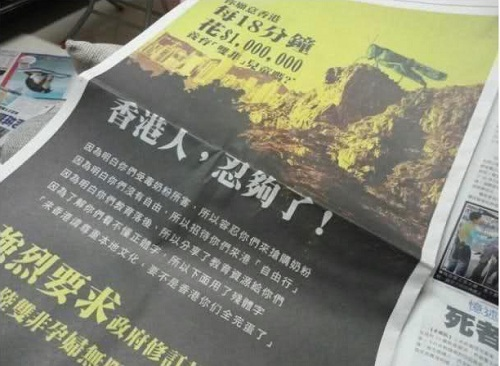
\includegraphics[width=3.3224in,height=2.4335in]{figures/chap2/chapitre2-img17.jpg}
    }
    \subfloat[Exemples de tracts réalisés par les internautes en réponse à la campagne]{
        % 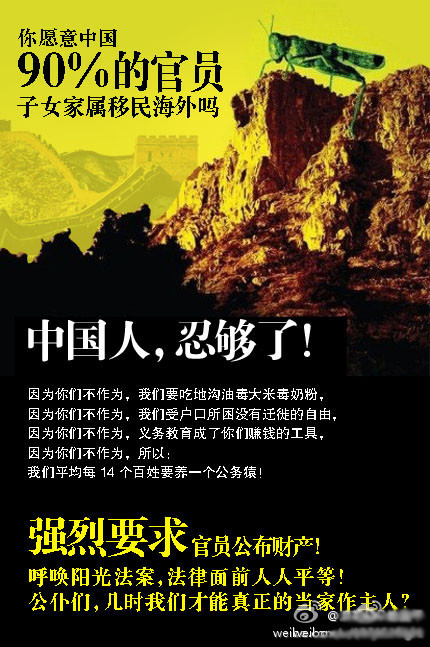
\includegraphics[width=1.4449in,height=2.178in]{figures/chap2/chapitre2-img18.jpg}
        
\includegraphics[width=1.4894in,height=2.1894in]{figures/chap2/chapitre2-img19.jpg}
        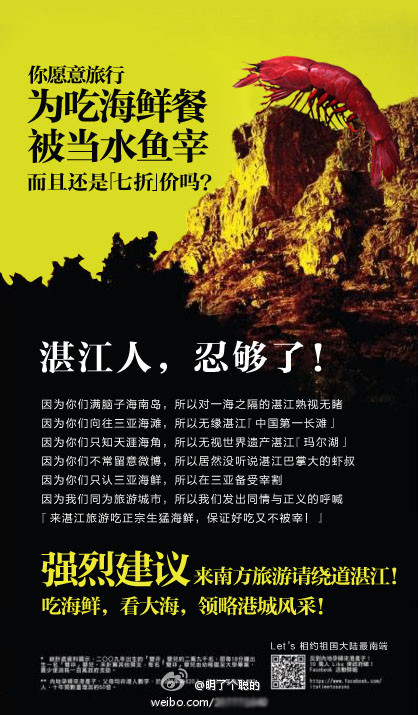
\includegraphics[width=1.2894in,height=2.2224in]{figures/chap2/chapitre2-img20.jpg}
        % 
\includegraphics[width=1.3669in,height=2.2114in]{figures/chap2/chapitre2-img21.jpg}
    }
    \caption[Détournement de tracts hongkongais anti-chinois]{Détournement de tracts hongkongais anti-chinois,d{\textquoteright}après \textit{The Civic Beat, }\url{http://reader.thecivicbeat.com/2012/03/locusts-and-pandas-and-bears-??-o-mai/} consulté le 1er Mars 2014 à 22h58}
    \label{fig:hk-tract}
\end{figure}

De nombreux chinois se rendent donc à Hong Kong pour voyager mais également profiter de la détaxe des produits de consommation et des services publics de bien meilleure qualité. La qualité des hôpitaux de la ville et l{\textquoteright}application du droit du sol dans la loi hongkongaise amènent de nombreuses jeunes mères venues de Chine à traverser la frontière pour venir accoucher à HK. Cette pratique très controversée donne à l{\textquoteright}enfant le passeport hongkongais et se monnaie à prix d{\textquoteright}or, rendant l{\textquoteright}accès aux hopitaux de plus en plus cher et attisant la colère des habitants de HK. En septembre 2012, une pétition lancée à Hongkong a cherché à recueillir des votes pour interdire l{\textquoteright}accès aux hôpitaux aux chinois venus de RPC. Un tract publié pour cette campagne a largement circulé sur le web chinois ; on pouvait y lire :\textit{ {\textquotedblleft}Habitants de Hong Kong, nous avons assez souffert ! (...) Ne nous laissons pas envahir par la vermine venue de Chine intérieure.{\textquotedblright}}  

Les internautes chinois choqués mais armés d{\textquoteright}un humour toujours très cinglant ont donc entamé une contre-campagne en proposant des versions modifiées et réécrites du dit tract. Réactions épidermiques, propos nationalistes sommaires, mais aussi critique du tourisme de masse, dénonciation de la corruption et de la mauvaise qualité des soins hospitaliers en Chine et nombreuses blagues absurdes, les adaptations et réponses singeant le tract d{\textquoteright}origine ont montré un panel d{\textquoteright}arguments et de réactions qui a permis de crever l{\textquoteright}abcés et d{\textquoteright}ouvrir un débat national sur ce problème épineux révélateur des griefs actuels des habitants de HK envers ceux de la RPC.  


\item[Fan clubs, adoration]
\hfill \\
Comme tout mass media, les réseaux sociaux possèdent une énorme quantité de contenus consacrés aux stars, à leurs vies, leurs coups durs et leurs derniers films et chansons. Développant des stratégies d{\textquoteright}envergure sur les médias chinois, de nombreuses stars internationales ont fait leur arrivée sur Sina Weibo comme notamment Brad Pitt ou Kobe Bryant. Néanmoins, leur influence reste incomparable à celles des stars originaires de Chine, de Taiwan et de Hong Kong ou bien encore de Corée du Sud, principal producteur de pop culture en Asie \citep{Martel2010}. Une des stars les plus plébiscitée dans les réseaux sociaux est pourtant une étrangère puisqu{\textquoteright}il s{\textquoteright}agit de la japonaise Sola Aoi, ex-actrice de film pornographique devenu une des 10 personnes les plus suivies sur Sina Weibo avec près de 15 millions de followers\footnote{ D{\textquoteright}après Sina Weibo \url{http://www.weibo.com/1739928273/yBJYNt7Ol,} consulté le 1 Mars 2017 à 23h11}. 

\begin{figure}[b]
    \centering
    
\includegraphics[scale=0.7]{figures/chap2/chapitre2-img22.jpg}
    \caption[La star du X japonaise Sola Aoi sur Sina Weibo]{Un message disant\textit{ {\textquotedblleft}Les peuples de la Chine et du Japon sont des amis{\textquotedblright} }posté par la star du cinéma pornographique japonaise Sola Aoi}
    \label{fig:pornstar-weibo}
\end{figure}

Personnalité médiatique publique, la star a depuis plusieurs années utilisé les réseaux sociaux pour nouer contact avec le public chinois qui semble bien la conna\^itre, malgré l{\textquoteright}interdiction de la pornographie en Chine. Aujourd{\textquoteright}hui retraitée du monde du X à 30 ans, Sola Aoi utilise sa popularité pour défendre une paix durable entre la Chine et le Japon. Alors que les tensions politiques exacerbées entre la Chine et le Japon ont mené à des rixes et des maltraitances envers les ressortissants dans les deux pays, elle a notamment contribué à créer un appel à la non-violence sous forme de mème \ qui a été extrêmement diffusé.  


Ainsi, les fan clubs et les stars elles-mêmes jouent un rôle important dans la création et la diffusion des mèmes, occupant une large place dans le paysage médiatique et notamment celui des réseaux sociaux. 


\item[Hoax, spam]
\hfill \\
\begin{figure}[ht]
    \begin{quote}
        I am Stella Amah 19 years of age the only daughter of late Mr Boni Amah whom was killed by the rebels that attacked our country cote d'Ivoire west Africa and took over our town (BOUAKE). I ran to Abidjan the economical capital of cote d'ivoire from were I am contacting you. Before the death of my father he told me that he has a sum of US\$9,000,000(Nine million united states dollars) kept in a private security company here in cote d'ivoire in my name as the next of kin... 
    \end{quote}
    \caption[Extrait d'un spam du type \textit{Nigerian Scam}]{
        Extrait d{\textquoteright}un {\textquotedblleft}Nigerian Scam{\textquotedblright}, d{\textquoteright}après \url{http://www.hoax-slayer.com/stella-amah-scam.shtml,} consulté le 2 Mars 2014 à 18h50
    }
    \label{fig:nigerian-scam}
\end{figure}

Un des plus célèbres exemples dans ce domaine sont les emails dits de {\textquotedblleft}fraude 4-1-9{\textquotedblright} cherchant à extorquer de l{\textquoteright}argent au destinataire. Le numéro 419 correspond au numéro de l{\textquoteright}article interdisant la pratique de l{\textquoteright}escroquerie en ligne dans le code pénal nigérian. En effet, la forme la plus connue de cette arnaque est celle du {\textquotedblleft}prince nigérian{\textquotedblright} demandant un numéro de compte bancaire pour y transférer rapidement des fonds. Adaptés sous de multiples formes, ce type de messages existent également sous les réseaux sociaux sous la forme de \textit{bots}, comptes tenus par des robots postant des messages promotionnels.  


\end{description}

Au regard des différents exemples données ici, nous voyons qu{\textquoteright}il est difficile de classer les mèmes selon des catégories précises et qu{\textquoteright}en bien des endroits ces catégories se recoupent : les stars font de la politique alors que les politiques font dans le comique. Ainsi, il ne s{\textquoteright}agit pas de dresser des catégories rigides mais de disposer d{\textquoteright}une classification flexible pour pouvoir analyser les éléments discursifs présents dans les mèmes Internet. La suite de cette étude interrogera plus précisément la constitution de ces formes de discursivités dans leurs multiples~empiriquement observables par l{\textquoteright}analyse de données issues de \textit{Sina Weibo}: structure du réseau social, contenu des mèmes, forme multimédia, éléments de contexte du message, etc. Nous allons donc maintenant présenter les méthodes d{\textquoteright}extraction, de traitement et d{\textquoteright}analyse de données en détaillant la méthodologie que nous avons retenue pour cette étude.